%%%%%%%%%%%%  Generated using docx2latex.com  %%%%%%%%%%%%%%

%%%%%%%%%%%%  v2.0.0-beta  %%%%%%%%%%%%%%

\documentclass[12pt]{report}
\usepackage{amsmath}
\usepackage{latexsym}
\usepackage{amsfonts}
\usepackage[normalem]{ulem}
\usepackage{array}
\usepackage{amssymb}
\usepackage{graphicx}
\usepackage[backend=biber,
style=numeric,
sorting=none,
isbn=false,
doi=false,
url=false,
]{biblatex}\addbibresource{bibliography.bib}

\usepackage{subfig}
\usepackage{wrapfig}
\usepackage{wasysym}
\usepackage{enumitem}
\usepackage{adjustbox}
\usepackage{ragged2e}
\usepackage[svgnames,table]{xcolor}
\usepackage{tikz}
\usepackage{longtable}
\usepackage{changepage}
\usepackage{setspace}
\usepackage{hhline}
\usepackage{multicol}
\usepackage{tabto}
\usepackage{float}
\usepackage{multirow}
\usepackage{makecell}
\usepackage{fancyhdr}
\usepackage[toc,page]{appendix}
\usepackage[hidelinks]{hyperref}
\usetikzlibrary{shapes.symbols,shapes.geometric,shadows,arrows.meta}
\tikzset{>={Latex[width=1.5mm,length=2mm]}}
\usepackage{flowchart}\usepackage[paperheight=11.69in,paperwidth=8.27in,left=1.77in,right=0.98in,top=0.98in,bottom=0.79in,headheight=1in]{geometry}
\usepackage[utf8]{inputenc}
\usepackage[T1]{fontenc}
\TabPositions{0.5in,1.0in,1.5in,2.0in,2.5in,3.0in,3.5in,4.0in,4.5in,5.0in,5.5in,}

\urlstyle{same}


 %%%%%%%%%%%%  Set Depths for Sections  %%%%%%%%%%%%%%

% 1) Section
% 1.1) SubSection
% 1.1.1) SubSubSection
% 1.1.1.1) Paragraph
% 1.1.1.1.1) Subparagraph


\setcounter{tocdepth}{5}
\setcounter{secnumdepth}{5}


 %%%%%%%%%%%%  Set Depths for Nested Lists created by \begin{enumerate}  %%%%%%%%%%%%%%


\setlistdepth{9}
\renewlist{enumerate}{enumerate}{9}
		\setlist[enumerate,1]{label=\arabic*)}
		\setlist[enumerate,2]{label=\alph*)}
		\setlist[enumerate,3]{label=(\roman*)}
		\setlist[enumerate,4]{label=(\arabic*)}
		\setlist[enumerate,5]{label=(\Alph*)}
		\setlist[enumerate,6]{label=(\Roman*)}
		\setlist[enumerate,7]{label=\arabic*}
		\setlist[enumerate,8]{label=\alph*}
		\setlist[enumerate,9]{label=\roman*}

\renewlist{itemize}{itemize}{9}
		\setlist[itemize]{label=$\cdot$}
		\setlist[itemize,1]{label=\textbullet}
		\setlist[itemize,2]{label=$\circ$}
		\setlist[itemize,3]{label=$\ast$}
		\setlist[itemize,4]{label=$\dagger$}
		\setlist[itemize,5]{label=$\triangleright$}
		\setlist[itemize,6]{label=$\bigstar$}
		\setlist[itemize,7]{label=$\blacklozenge$}
		\setlist[itemize,8]{label=$\prime$}



 %%%%%%%%%%%%  Header here  %%%%%%%%%%%%%%


\pagestyle{fancy}
\fancyhf{}
\cfoot{ \setlength{\parskip}{0.0pt}
}
\renewcommand{\headrulewidth}{0pt}
\setlength{\topsep}{0pt}\setlength{\parindent}{0pt}
\renewcommand{\arraystretch}{1.3}


%%%%%%%%%%%%%%%%%%%% Document code starts here %%%%%%%%%%%%%%%%%%%%



\begin{document}
\begin{Center}
CMPUT 414 
\end{Center}\par

\begin{Center}
Introduction to Multimedia Technology
\end{Center}\par


\vspace{\baselineskip}

\vspace{\baselineskip}

\vspace{\baselineskip}

\vspace{\baselineskip}

\vspace{\baselineskip}

\vspace{\baselineskip}

\vspace{\baselineskip}

\vspace{\baselineskip}

\vspace{\baselineskip}
\begin{Center}
Final Report
\end{Center}\par

\begin{Center}
LiDAR Data Analysis
\end{Center}\par


\vspace{\baselineskip}

\vspace{\baselineskip}

\vspace{\baselineskip}

\vspace{\baselineskip}

\vspace{\baselineskip}

\vspace{\baselineskip}

\vspace{\baselineskip}

\vspace{\baselineskip}

\vspace{\baselineskip}
\begin{Center}
Submitted by
\end{Center}\par


\vspace{\baselineskip}
\begin{Center}
Sangaré, Ibrahima
\end{Center}\par

\begin{Center}
Uddin, Fahmid
\end{Center}\par


\vspace{\baselineskip}

\vspace{\baselineskip}

\vspace{\baselineskip}

\vspace{\baselineskip}

\vspace{\baselineskip}

\vspace{\baselineskip}

\vspace{\baselineskip}

\vspace{\baselineskip}

\vspace{\baselineskip}

\vspace{\baselineskip}

\vspace{\baselineskip}

\vspace{\baselineskip}

\vspace{\baselineskip}

\vspace{\baselineskip}
\begin{Center}
Saturday April 27th 2019
\end{Center}\par


\vspace{\baselineskip}

\vspace{\baselineskip}

\vspace{\baselineskip}

\vspace{\baselineskip}

\vspace{\baselineskip}

\vspace{\baselineskip}

\vspace{\baselineskip}

\vspace{\baselineskip}

\vspace{\baselineskip}

\vspace{\baselineskip}

\vspace{\baselineskip}

\vspace{\baselineskip}

\vspace{\baselineskip}

\vspace{\baselineskip}

\vspace{\baselineskip}


 %%%%%%%%%%%%  This Produces Table Of Contents %%%%%%%%%%%%%%

\tableofcontents
\addcontentsline{toc}{chapter}{Contents}

\vspace{\baselineskip}

\vspace{\baselineskip}

\vspace{\baselineskip}

\vspace{\baselineskip}

\vspace{\baselineskip}

\vspace{\baselineskip}

\vspace{\baselineskip}

\vspace{\baselineskip}

\vspace{\baselineskip}

\vspace{\baselineskip}

\vspace{\baselineskip}

\vspace{\baselineskip}

\vspace{\baselineskip}

\vspace{\baselineskip}

\vspace{\baselineskip}

\vspace{\baselineskip}

\vspace{\baselineskip}

\vspace{\baselineskip}

\vspace{\baselineskip}

\vspace{\baselineskip}

\vspace{\baselineskip}

\vspace{\baselineskip}

\vspace{\baselineskip}

\vspace{\baselineskip}

\vspace{\baselineskip}

\vspace{\baselineskip}

\vspace{\baselineskip}

\vspace{\baselineskip}

\vspace{\baselineskip}

\vspace{\baselineskip}

\vspace{\baselineskip}

\vspace{\baselineskip}

\vspace{\baselineskip}

\vspace{\baselineskip}

\vspace{\baselineskip}

\vspace{\baselineskip}

\vspace{\baselineskip}

\vspace{\baselineskip}

\vspace{\baselineskip}

\vspace{\baselineskip}

\vspace{\baselineskip}
\paragraph*{Introduction}
\addcontentsline{toc}{paragraph}{Introduction}

\vspace{\baselineskip}
LiDAR stands for Light Detection And Ranging \footnote{ "What is LIDAR? - NOAA's National Ocean Service." https://oceanservice.noaa.gov/facts/lidar.html. Accessed 13 Apr. 2019. }. It works by projecting laser light pulses onto surfaces, which then reflects a signal captured as energy to the device. Target objects are then identified based on their coordinates in a 3D space from a certain range. The measuring device is made of several components including a laser, sensors, scanners, navigation systems, etc... It can different forms: airborne, satellite-borne, terrestrial-based or drone-based [12]. In the context of building reconstruction, airborne-based LiDAR is frequently used to capture data for further processing. LiDAR produces a point cloud that represents the surroundings. Depending on the filtering applied to the point cloud, it is possible to produces Digital Terrain Models (DTMs), Digital Surface Models (DSMs) and Digital Elevation Models (DEMs) which are all ways to model elevation in specific region. These models have applications for vegetation management (DTMs), terrain stability and, soil mapping (DEMs) [13]. It has recently become a popular method of gathering data as self-driving cars and machine learning turned more mainstream. Its most common implementation is generally found in building reconstruction, forestry, and agriculture. LiDAR has been getting more and more attention in the machine learning in recent years and should lead to interesting improvement in future technology. \par


\vspace{\baselineskip}
Practically, researchers most often use the following framework for 3D reconstruction purposes [].\par


\vspace{\baselineskip}


%%%%%%%%%%%%%%%%%%%% Figure/Image No: 1 starts here %%%%%%%%%%%%%%%%%%%%

\begin{figure}[H]
	\begin{Center}
		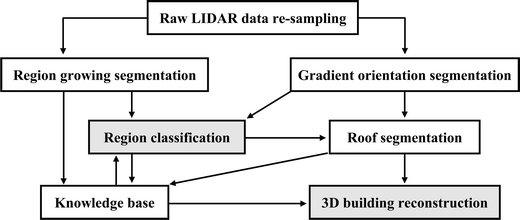
\includegraphics[width=5.42in,height=2.29in]{./media/image6.png}
	\end{Center}
\end{figure}


%%%%%%%%%%%%%%%%%%%% Figure/Image No: 1 Ends here %%%%%%%%%%%%%%%%%%%%

\par


\vspace{\baselineskip}
\begin{Center}
\textbf{Figure 1}: Proposed framework for 3D building Reconstruction.
\end{Center}\par


\vspace{\baselineskip}
The idea behind the framework is to interpolate LiDAR data over a grid which is further dissected into regions by using 3D reconstruction algorithms. Segmentation is applied to form a knowledge base that is used to reconstruct the desired objects [8].\par

.\par

The main theme of this project is based around the concept of 3D reconstruction. As mentioned above, we aimed to use LiDAR for reconstruction. In this project, our aim was to provide a tool that would be able to analyze LiDAR Data from real-word scanned objects with a Lidar scanner provided by the University of Alberta. It would be a convenient and efficient way to visualize data using powerful graphical libraries from the Python language. We are tackling In this report, we will discuss the importance of LiDAR technology as well as it uses and benefits in tackling problems in 3D reconstruction, related work in the scientific literature, our methods and implementation, our results and a brief conclusion.\par


\vspace{\baselineskip}
\paragraph*{Review of Existing Work}
\addcontentsline{toc}{paragraph}{Review of Existing Work}

\vspace{\baselineskip}
\textbf{Existing 3D Reconstruction Algorithms\tab }\par


\vspace{\baselineskip}
There are three general methods employed in 3D reconstruction. Random Sampling Consensus (RANSAC) is the most commonly used in reconstruction. Hough transform and region growing (which is an encapsulating term and has many different forms depending on the research group) are also used to a lesser extent [8]. On one hand, the RANSAC algorithm is used for roof modelling and is useful to accurately represent the building’s shape. It operates on a set of random points gathered from the point cloud and finds a model that represents the dataset. The model is improved iteratively by testing other points from the point cloud against the model to identify its weaknesses. On the other hand, Hough transform is a known mathematical principle that has been used in image processing to be able to detect geometric primitives. Building contours are identifiable by this technique. This algorithm relies on a $``$parameter space$"$  representation of the point cloud data and tries to find the best planes to represent the points. It is statistically driven and thus is not ultimately grounded in reality, nor is it always practical when it comes to determining the shape of the building. Even though the results are generally accurate, Tarsha-Kurdi et al. have found through thorough testing of both methods over large datasets, that RANSAC is a faster, more effective algorithm in the context of 3D reconstruction in most cases [2].\tab \par


\vspace{\baselineskip}
\textbf{Existing Methods for LiDAR 3D Reconstruction}\par


\vspace{\baselineskip}
\textbf{Applications and Importance of LiDAR}\par


\vspace{\baselineskip}
High level tasks such as city planning or analysis of building structures require a level of sophistication that will make this task as efficient as possible. These fields leverage the power of LiDAR and point clouds, to make 3D reconstructions of materials that are required for the study. This is just \textit{one} out of several potential uses for this revolutionary tech.\par


\vspace{\baselineskip}
The technique of creating polygons, cylinders or basically any other shapes to build out an explorable map of our environment is particularly a very interesting method for forest science. The use of terrestrial LiDAR (light detection and ranging) scanners in forest environments is being studied extensively at present due to the high potential of this technology to acquire three-dimensional data on standing trees rapidly and accurately [5]. Further, This means that point clouds can be used to map out forests and the trees it encloses. Therefore, the data generated by this process saves a lot of time for researchers studying these forests.\par


\vspace{\baselineskip}
The figure below shows how voxels are used on the point clouds to generate geometric objects to best fit those data points. First we establish a digital terrain model (DTM) created from the point cloud, which is the basis for further parameter extraction [5]. Then the points are separated with grids, which is then used to create 3D objects with best fitting (this math involved least squares) - resulting in 3D reconstruction from point cloud.\par


\vspace{\baselineskip}


%%%%%%%%%%%%%%%%%%%% Figure/Image No: 2 starts here %%%%%%%%%%%%%%%%%%%%

\begin{figure}[H]
	\begin{Center}
		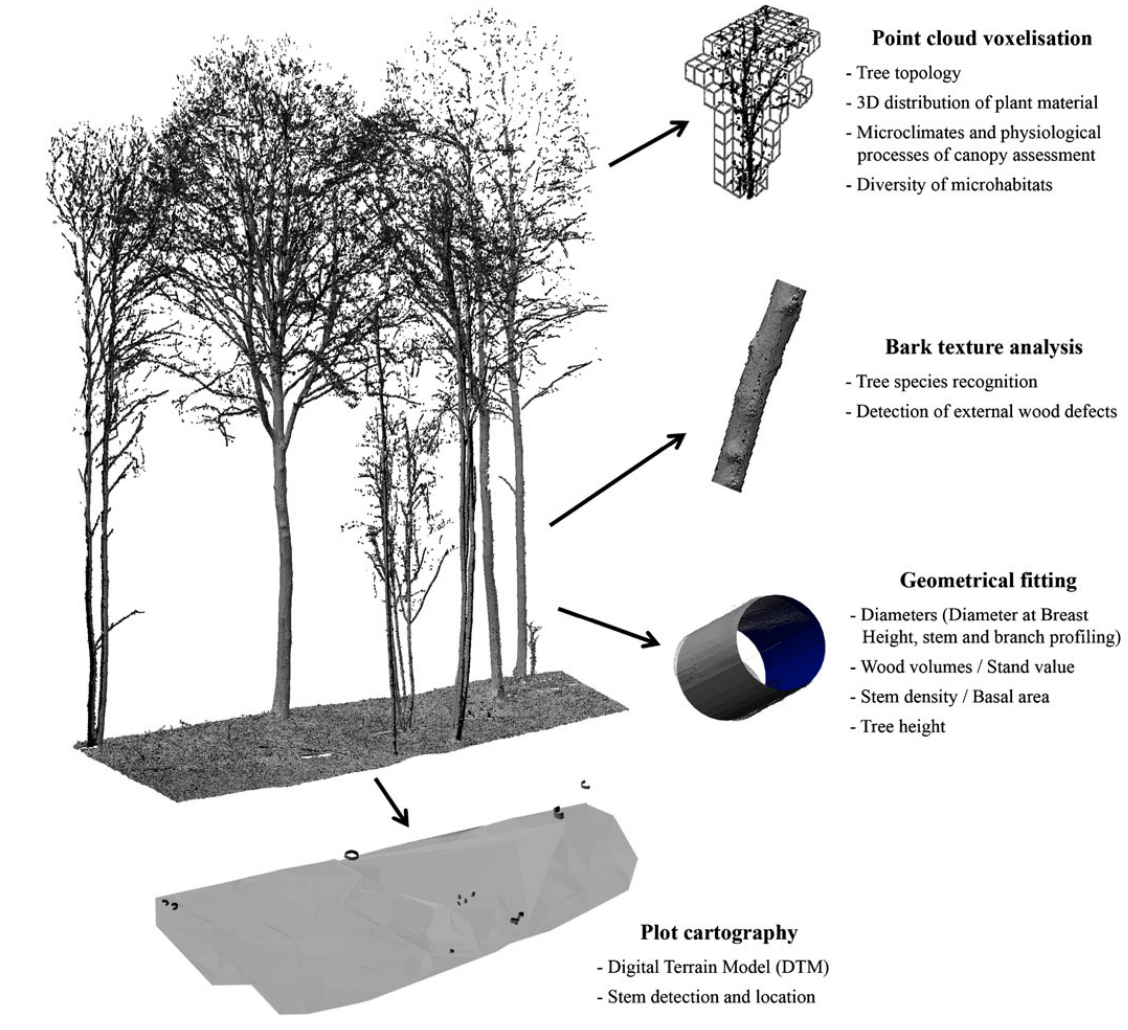
\includegraphics[width=2.66in,height=2.46in]{./media/image14.png}
	\end{Center}
\end{figure}


%%%%%%%%%%%%%%%%%%%% Figure/Image No: 2 Ends here %%%%%%%%%%%%%%%%%%%%

\begin{Center}
 [5]
\end{Center}\par

\begin{Center}
\textbf{Figure 2}: Object generation process.
\end{Center}\par


\vspace{\baselineskip}
\textbf{LiDAR in Dynamic Locations}\par


\vspace{\baselineskip}
While mapping out forests and trees is one challenge, creating an entire 3D map of buildings or cities is another game. There are a few methods to do this, such as reconstruction based on cell decomposition approach, analyzing geometric properties of the area to create wireframes, and many others.\par


\vspace{\baselineskip}
A spatial partitioning representation in solid modelling, where solids are decomposed into non intersecting, typically parameterized primitives, is called cell decomposition [1]. This method can be very useful when turning point clouds of buildings into 3D models. Although one pair of images, using photogrammetry, is adequate to find the 3D position of two corresponding and visible image features; it is not sufficient to extract the entire building due to hidden parts of the building that are not seen in the image pair [4]. That is a good observation that can be tackled using the method of cell decomposition. Since it uses roofs as one of the key methods to convert the data into 3D, partial data of the buildings can be made use to serve its purpose. If the surface model is structured as a grid, we compute the normal vector of each point from the eight triangles fanned around it and average their normal vectors [1]. However, if the raw data is available in form of an unstructured point cloud, we estimate a point’s local plane of regression from its five nearest neighbours and take the resulting surface normal vector [1]. These are some methods by how urban area point clouds are converted to 3D meshes.\par


\vspace{\baselineskip}

\vspace{\baselineskip}
\textbf{3D Feature Extraction}\par


\vspace{\baselineskip}
With the availability of many sources of data such as conventional imagery, SAR imaging, IFSAR DEMs, and LIDAR DEMs, there are many avenues open to derive terrain and feature data in urban areas [3]. Extracting features from normal imagery is quite different from the way it’s done with point clouds. An advantage of LiDAR is that the echo system this technology uses not only bounces back at the surface of the targeted object(s), but also penetrates beyond it in certain cases. This can be used to analyse the data even further and make use of that \textit{intensity} to create all sorts of maps and 3D environments. LiDAR uses laser beams to create echos which comes back to the source with useful data such as location and intensity. Let’s take a surface for example. When the laser beam hits the exposed surface it will have a footprint with a size in the range of 15-30 cm or more [3]. So, if the laser beam hits the edge of a building then part of the beam footprint will be reflected from the top roof of the building and the other part might reach the ground [3]. This observation allows us to plug those data in the equation below to find the height of buildings.\par



%%%%%%%%%%%%%%%%%%%% Figure/Image No: 3 starts here %%%%%%%%%%%%%%%%%%%%

\begin{figure}[H]
	\begin{Center}
		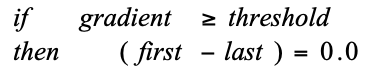
\includegraphics[width=2.31in,height=0.41in]{./media/image1.png}
	\end{Center}
\end{figure}


%%%%%%%%%%%%%%%%%%%% Figure/Image No: 3 Ends here %%%%%%%%%%%%%%%%%%%%

\par


\vspace{\baselineskip}
A color coded map can then be generated for further studies.\par


\vspace{\baselineskip}


%%%%%%%%%%%%%%%%%%%% Figure/Image No: 4 starts here %%%%%%%%%%%%%%%%%%%%

\begin{figure}[H]
	\begin{Center}
		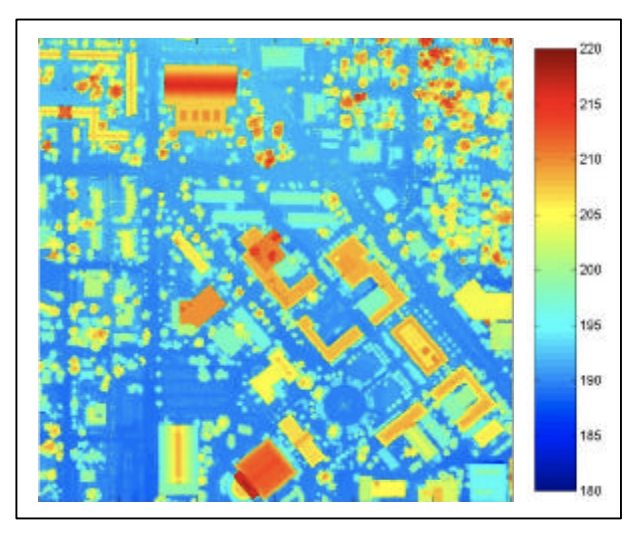
\includegraphics[width=3.54in,height=2.96in]{./media/image12.png}
	\end{Center}
\end{figure}


%%%%%%%%%%%%%%%%%%%% Figure/Image No: 4 Ends here %%%%%%%%%%%%%%%%%%%%

\begin{Center}
 
\end{Center}\par

\tab \tab \textbf{Figure 3}: Color coded map from gradient calculation.\par


\vspace{\baselineskip}
\paragraph*{Methods}
\addcontentsline{toc}{paragraph}{Methods}
\tab In order to build our visualizing app, we first explored the possibility of using Blender. Blender is a an Open Source 3D creation software that supports Python scripting. It is widely used for all things related to 3D animation, modeling, rendering, reconstruction, etc.. \par


\vspace{\baselineskip}


%%%%%%%%%%%%%%%%%%%% Figure/Image No: 5 starts here %%%%%%%%%%%%%%%%%%%%

\begin{figure}[H]
	\begin{Center}
		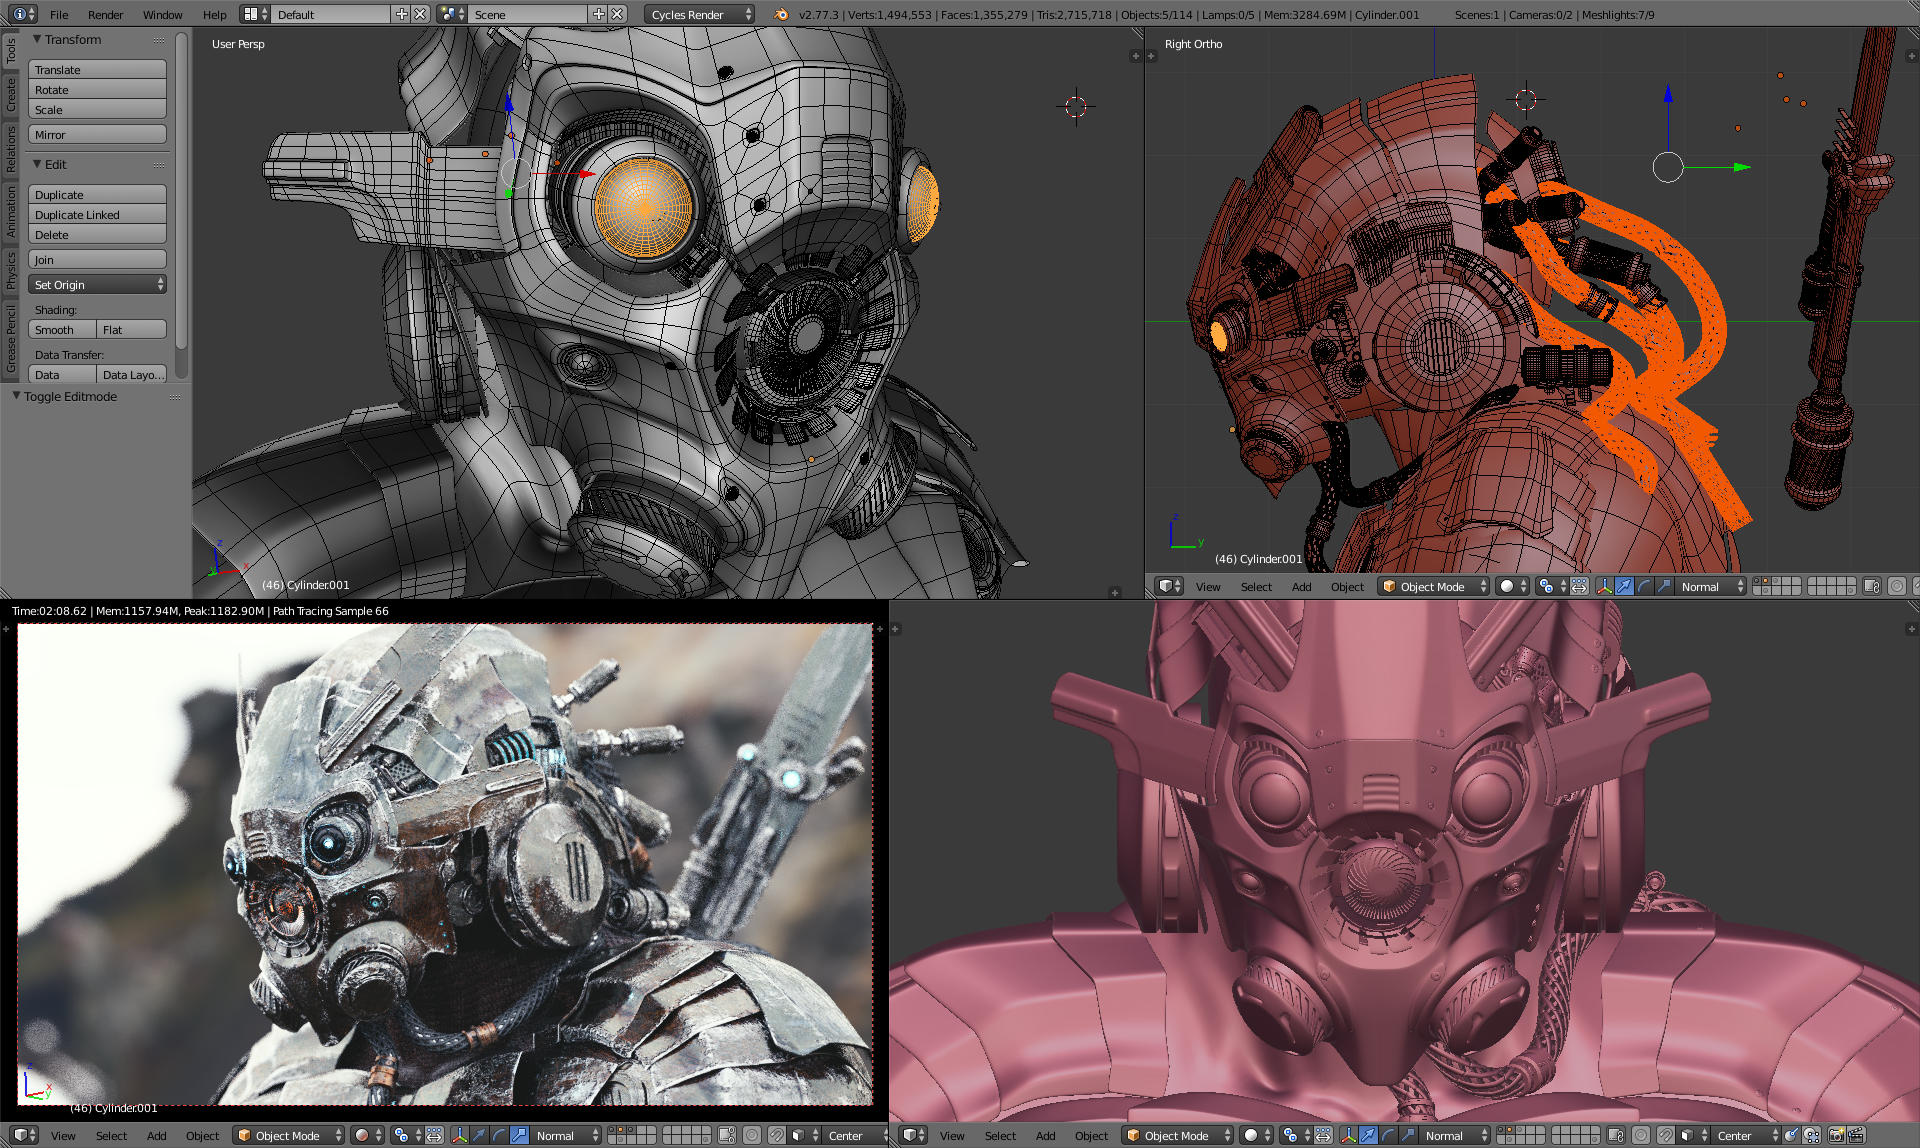
\includegraphics[width=5.51in,height=3.29in]{./media/image16.png}
	\end{Center}
\end{figure}


%%%%%%%%%%%%%%%%%%%% Figure/Image No: 5 Ends here %%%%%%%%%%%%%%%%%%%%

\tab \par


\vspace{\baselineskip}
\begin{Center}
\textbf{Figure 4: }Illustration of Blender 3D model.
\end{Center}\par


\vspace{\baselineskip}
\begin{FlushLeft}
The objective was to produce an app similar to this feature made available by the 3D modeling tool called Sketchfab.
\end{FlushLeft}\par



%%%%%%%%%%%%%%%%%%%% Figure/Image No: 6 starts here %%%%%%%%%%%%%%%%%%%%

\begin{figure}[H]
	\begin{Center}
		\includegraphics[width=5.51in,height=2.88in]{./media/image15.gif}
	\end{Center}
\end{figure}


%%%%%%%%%%%%%%%%%%%% Figure/Image No: 6 Ends here %%%%%%%%%%%%%%%%%%%%

\par

\begin{Center}
\textbf{Figure 5}: Sketchfab feature to edit Lidar Data.
\end{Center}\par


\vspace{\baselineskip}
\begin{FlushLeft}
We decided to use the open source Python library called Kivy to create an app capable of providing a similar layout to the app above. Kivy is a cross platform library that can be used on Android, Linux, Windows, OS X and Raspberry Pi. This makes the app portable without making any changes to the code and only adding a few configuration files to the project depending on the operating system. Python is good language for the task due to simplicity, portability and its number of libraries for computer graphics. 
\end{FlushLeft}\par

\begin{FlushLeft}
The process of acquiring a LiDAR data was done with the help Dr. Arturo Sanchez and Professor Anup Basu. We were able to collect data with equipment provided by the University using a LiDAR device. The data was stored in a text file that could be later converted to any desired format (PLY, OBJ, LAS). The rest of our methods does not rely upon complex algorithms for visualization as python libraries facilitated this aspect of the project.
\end{FlushLeft}\par

\paragraph*{Implementation}
\addcontentsline{toc}{paragraph}{Implementation}

\vspace{\baselineskip}
\tab In this part, we take an in-depth look to all of implementation details that allowed us to come up with an interesting tool for analyzing LiDAR data. First, the app, as most Kivy based apps, there are two files needed for a working project. There is a KV file and a Python file for the graphical layout of the app and the logic behind the app, respectively. One difference between those two files is that, the KV file uses a syntax that is specific to Kivy. It is also important to note that the Kivy file is and should be named after the main class of the project (the one that inherits from the App class from Kivy’s module). \par


\vspace{\baselineskip}
\textbf{KV File}\par

\tab 
\vspace{\baselineskip}When we take a look at the content of the KV file, there are a collection of classes representing visual items in the app. Each class definition with quotation marks represent a custom class that is defined to implement objects with and id and additional attributes. There are thus custom classes named \textit{Separator, Misc, GroundColor, BackColor, PointColor, Viewer, Analyzer.}\par


\vspace{\baselineskip}
\tab All the classes with Color attached to the name are designed to have widgets that modify the color of an object that is a part of the scene displaying the LiDAR data. The app is laid out into a drawer defined as an \textit{Accordion} that contains settings to alter the data. There are five sections to the drawer called \textit{AccordionItem}. The first \textit{AccordionItem }is called $``$Point Cloud$"$  and contains sliders to change point cloud size and color. The second \textit{AccordionItem, }$``$Background Color$"$ \textit{ }contains sliders and text inputs to change background color. The $``$Ground Color$"$  \textit{AccordionItem} has the same content but affects the ground color. The $``$Misc$"$  \textit{AccordionItem }contains three checkboxes that can enable or disable the display positional information from the camera or the 3D Axis. The last \textit{AccordionItem, }$``$Floor Level$"$ , has a slider that can adjust the level of the floor relative to where the point clouds seat in the scene.\par


\vspace{\baselineskip}
All of these classes are contained in the \textit{Analyzer }class that is basically the entry point to the app’s content. Additionally, there is an \textit{ActionBar }at the top of the window for either exiting the app or import LiDAR data. The following figures can further illustrate where the components of the app seats in relation to one another.\par


\vspace{\baselineskip}
There is also a section dedicated to instructions on how to use the viewer and some guidelines.\par


\vspace{\baselineskip}


%%%%%%%%%%%%%%%%%%%% Figure/Image No: 7 starts here %%%%%%%%%%%%%%%%%%%%


\begin{figure}[H]	\begin{subfigure}		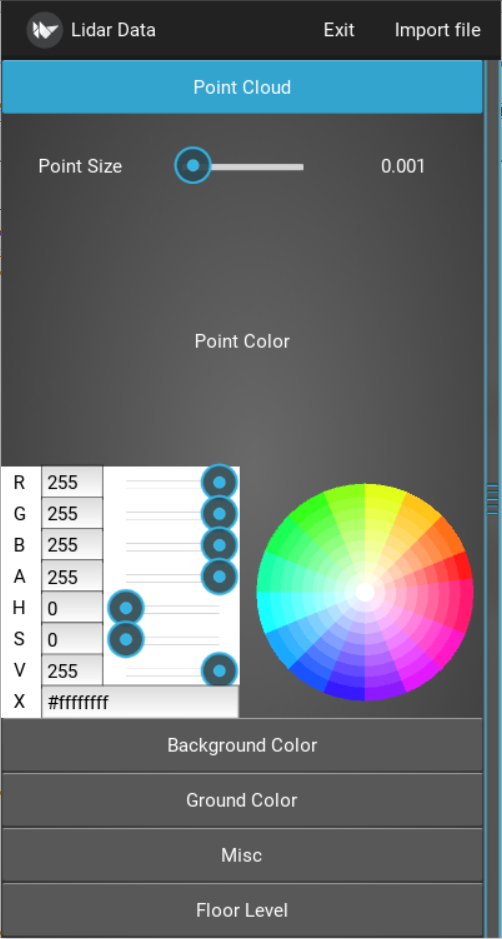
\includegraphics[width=0.45\textwidth]{./media/image3.png}
	\end{subfigure}
~	\begin{subfigure}		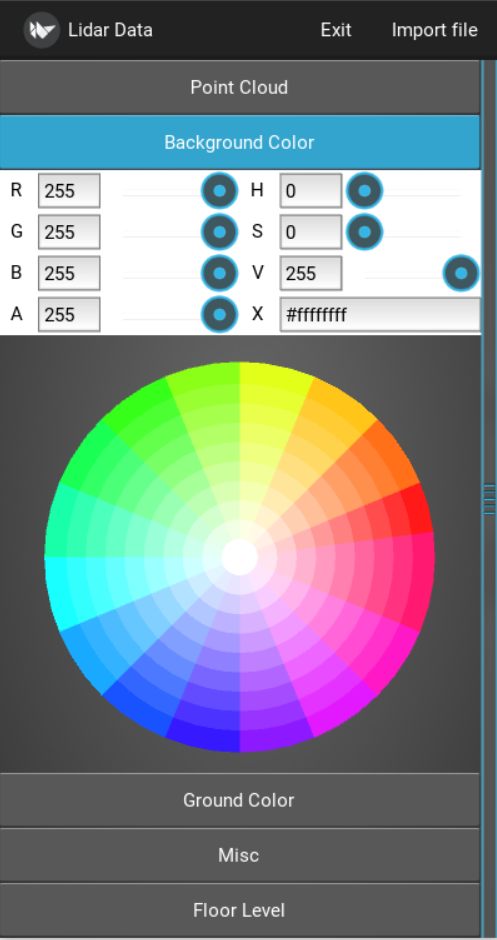
\includegraphics[width=0.45\textwidth]{./media/image2.png}
	\end{subfigure}
~
\end{figure}


%%%%%%%%%%%%%%%%%%%% Figure/Image No: 7 Ends here %%%%%%%%%%%%%%%%%%%%

\par


\vspace{\baselineskip}
\begin{Center}
\textbf{Figure 6: }Point cloud and background color accordion items.
\end{Center}\par



%%%%%%%%%%%%%%%%%%%% Figure/Image No: 8 starts here %%%%%%%%%%%%%%%%%%%%


\begin{figure}[H]	\begin{subfigure}		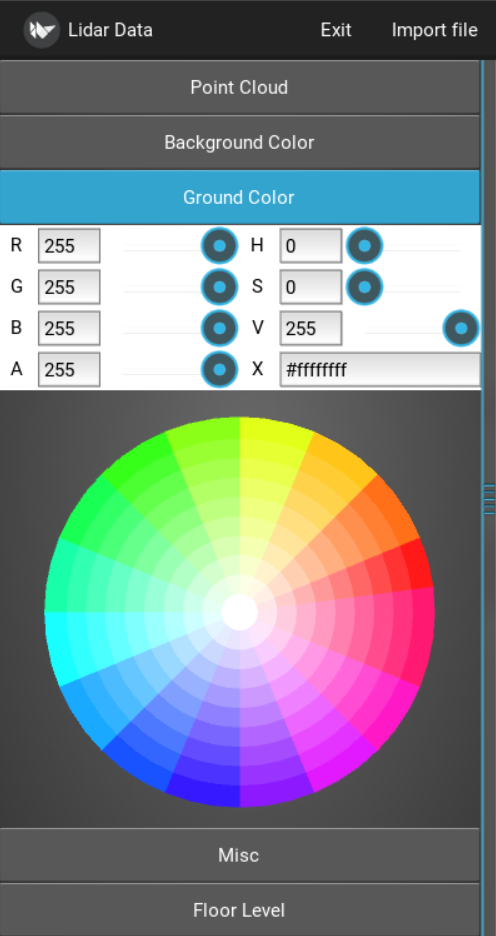
\includegraphics[width=0.45\textwidth]{./media/image13.png}
	\end{subfigure}
~	\begin{subfigure}		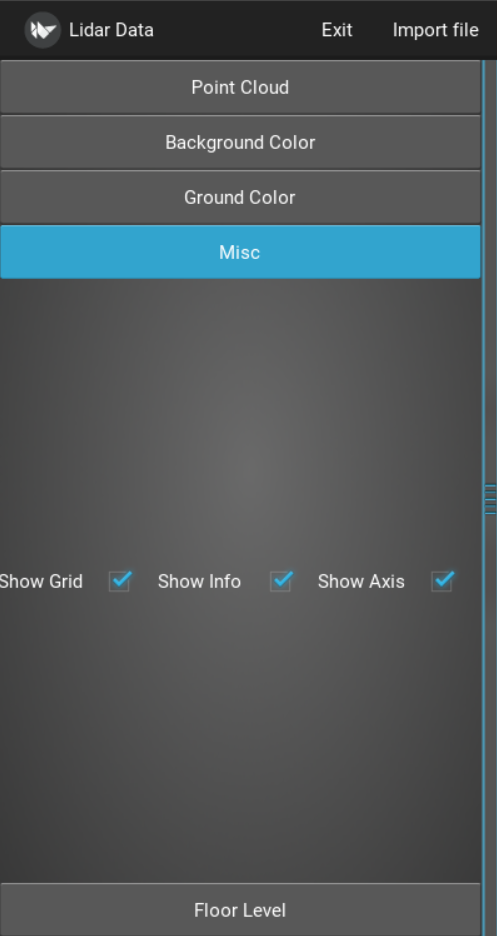
\includegraphics[width=0.45\textwidth]{./media/image9.png}
	\end{subfigure}
~
\end{figure}


%%%%%%%%%%%%%%%%%%%% Figure/Image No: 8 Ends here %%%%%%%%%%%%%%%%%%%%

\par


\vspace{\baselineskip}
\begin{Center}
\textbf{Figure 7: }Ground color and background color accordion items.
\end{Center}\par


\vspace{\baselineskip}

\vspace{\baselineskip}


%%%%%%%%%%%%%%%%%%%% Figure/Image No: 9 starts here %%%%%%%%%%%%%%%%%%%%


\begin{figure}[H]	\begin{subfigure}		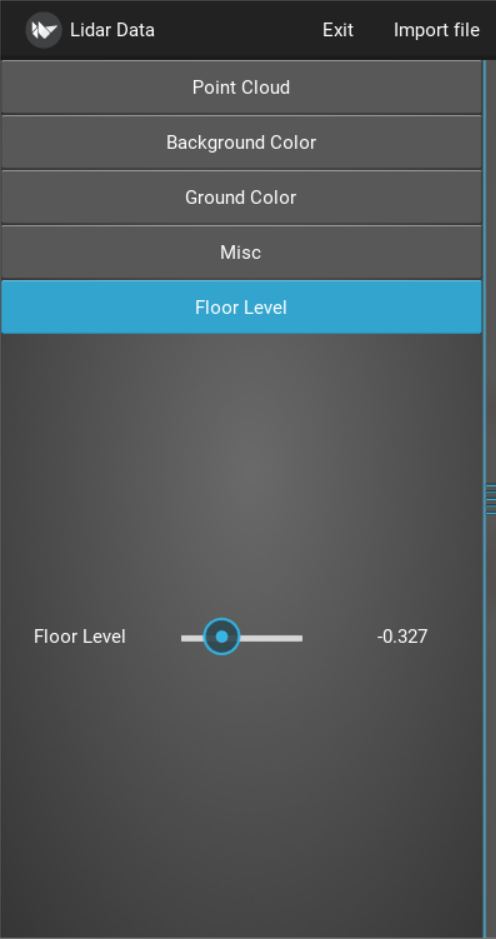
\includegraphics[width=0.45\textwidth]{./media/image5.png}
	\end{subfigure}
~	\begin{subfigure}		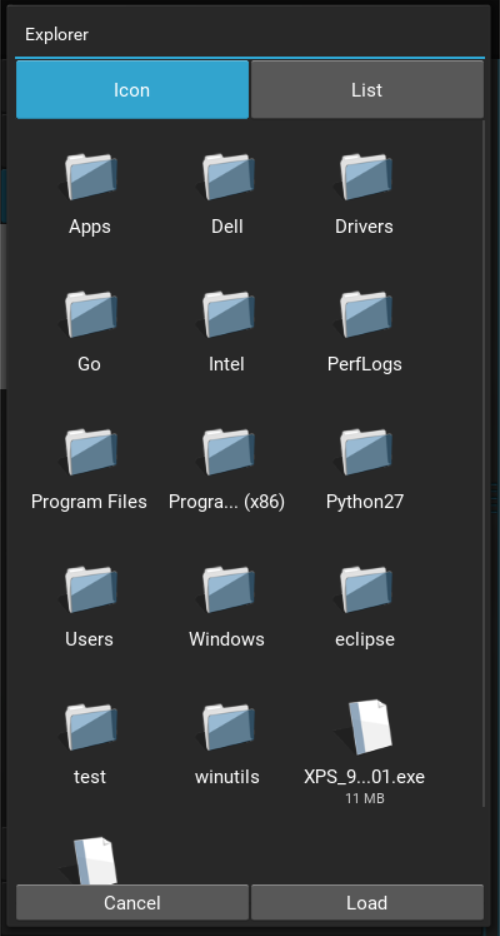
\includegraphics[width=0.45\textwidth]{./media/image8.png}
	\end{subfigure}
~
\end{figure}


%%%%%%%%%%%%%%%%%%%% Figure/Image No: 9 Ends here %%%%%%%%%%%%%%%%%%%%

\par


\vspace{\baselineskip}

\vspace{\baselineskip}
\begin{Center}
\textbf{Figure 8: }Floor level accordion item and explorer.
\end{Center}\par



%%%%%%%%%%%%%%%%%%%% Figure/Image No: 10 starts here %%%%%%%%%%%%%%%%%%%%


\begin{figure}[H]	\begin{subfigure}		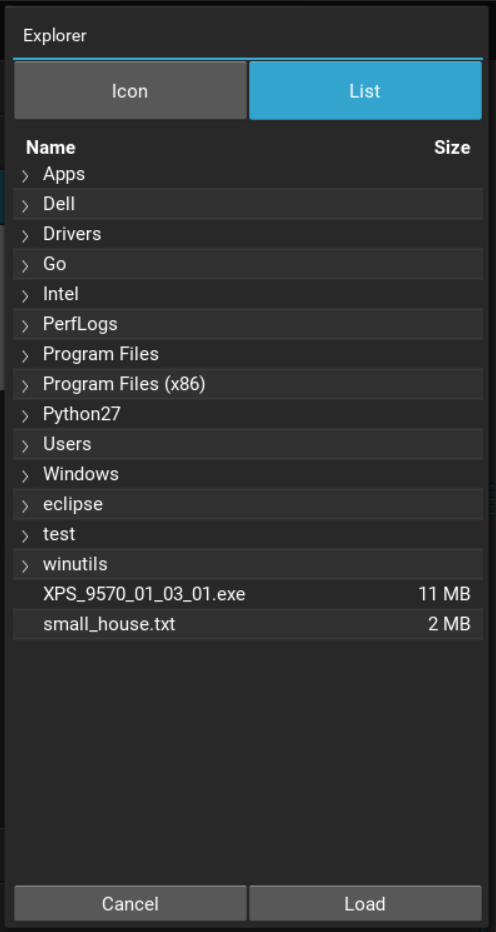
\includegraphics[width=0.45\textwidth]{./media/image4.png}
	\end{subfigure}
~	\begin{subfigure}		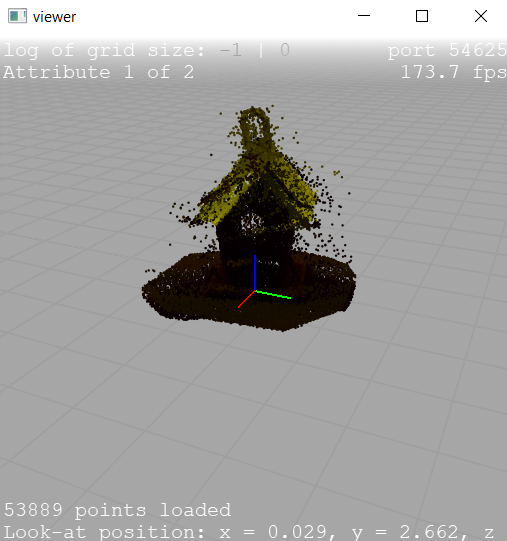
\includegraphics[width=0.45\textwidth]{./media/image10.png}
	\end{subfigure}
~
\end{figure}


%%%%%%%%%%%%%%%%%%%% Figure/Image No: 10 Ends here %%%%%%%%%%%%%%%%%%%%

\par


\vspace{\baselineskip}

\vspace{\baselineskip}
\begin{Center}
\textbf{Figure 9: }Second view of explorer and viewer.
\end{Center}\par


\vspace{\baselineskip}


%%%%%%%%%%%%%%%%%%%% Figure/Image No: 11 starts here %%%%%%%%%%%%%%%%%%%%

\begin{figure}[H]
	\begin{Center}
		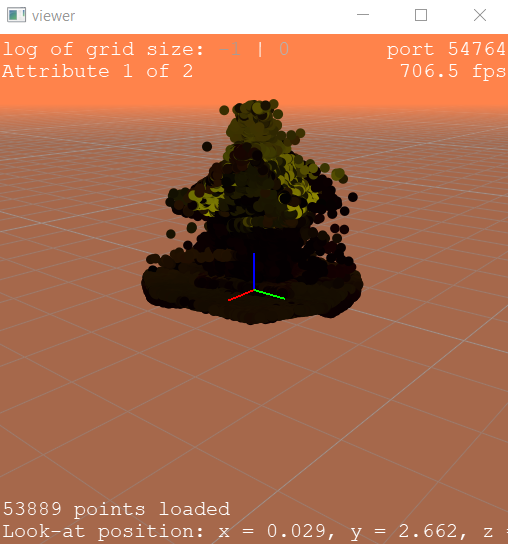
\includegraphics[width=5.29in,height=5.67in]{./media/image7.png}
	\end{Center}
\end{figure}


%%%%%%%%%%%%%%%%%%%% Figure/Image No: 11 Ends here %%%%%%%%%%%%%%%%%%%%

\par


\vspace{\baselineskip}
\begin{Center}
\textbf{Figure 10: }Alterations to point cloud size and background color.
\end{Center}\par


\vspace{\baselineskip}

\vspace{\baselineskip}
\begin{FlushLeft}
\textbf{Python File}
\end{FlushLeft}\par

\tab 
\vspace{\baselineskip}\begin{FlushLeft}
\tab The python file basically implements the logic behind all the widgets inside the app. The main app is the \textit{PointCloudAnalyzerApp }class, even though it does not contain the important functions of the program. It is there to only launch the Kivy app.
\end{FlushLeft}\par


\vspace{\baselineskip}
\begin{FlushLeft}
\tab First, we should consider the imports that are essential to the program. In order to have a viewer that can process the LiDAR, we use the pptk, pandas and numpy modules. The os module allows to import files from the device that is running the app. The rest of the imported classes are import from the Kivy module including App, Clock, ObjectProperty, Button, BoxLayout, Widget, Popup, ColorPicker, Factory, Color, Point, Checkbox, Label, and Config.
\end{FlushLeft}\par


\vspace{\baselineskip}
\begin{FlushLeft}
The App class does what the name implies by providing a stock class to run a Kivy app. The ObjectProperty class defines a property that is linked to a Kivy widget. The Button class is a class that allows to put clickable buttons in the app. The BoxLayout is a type of layout that places the elements inside the app in a vertical or horizontal fashion, one after the other. The Widget class is the parent class to all Widgets and can be used if the type of widget is not known in advance. The Popup serves to create popups when a new window is not needed and just a dialog might suffice for the current context. The ColorPicker provides an ergonomic interface to be able to change the color of the point clouds in our app. The Factory class allows to register certain classes that can make it easier to find certain objects or widgets in the app when coding or when many widgets are embedded into another widget.The Color class allows to create a tuple containing RGB and alpha values to change point cloud, background and ground color. The Chekbox and Label are self explanatory widgets. The Config import serves to adjust parameters of the window that contains the app.
\end{FlushLeft}\par


\vspace{\baselineskip}
\begin{FlushLeft}
The first functions inside the program are functions that are bound to changes that occur in the app. These changes can be changes made to the background, ground, point cloud, floor or the viewer. These functions are supposed to propagate the changes in color, size and display. They are the following: \textit{BackColorChange, GroundColorChange, PointColorChange, OnPointSizeChange, OnFloorSizeChange, OnFloorChange, gridActive, gridActive, infoActive, }and \textit{axisActive}. 
\end{FlushLeft}\par


\vspace{\baselineskip}
\begin{FlushLeft}
The \textit{Misc }class is represents the \textit{AccordionItem }and organizes the content of that item by placing it inside a BoxLayout with widgets. The same is true for the \textit{GroundColor, PointColor, }and \textit{BackColor}. The main class has a BoxLayout with all the other classes mentioned above to populate the app.\textit{ }There are functions to be able to read LiDAR files, load them, or save changes made to the data. One final function allows to dismiss pop ups when the app is running.
\end{FlushLeft}\par


\vspace{\baselineskip}
\paragraph*{Results}
\addcontentsline{toc}{paragraph}{Results}
\tab 
\vspace{\baselineskip}\begin{FlushLeft}
In comparison to the objective we set out to accomplish in the beginning, we think we were able to achieve our goal of providing a user friendly tool that would allow quick and effective visualization of LiDAR data. When we compare the functionalities of our app to the example provided in the proposal, we think that our app is relatively close in that aspect with, perhaps, a few subtleties in certain functionalities. The core functionalities are very stable and give us a framework to expand upon in the future. The tool we built has a lower quality in terms of display due to the limitations on the data and library we have used. Nevertheless, the shapes formed by the point cloud is accurate enough to provide clear shapes of the scanned object.
\end{FlushLeft}\par


\vspace{\baselineskip}


%%%%%%%%%%%%%%%%%%%% Figure/Image No: 12 starts here %%%%%%%%%%%%%%%%%%%%


\begin{figure}[H]	\begin{subfigure}		\includegraphics[width=0.45\textwidth]{./media/image15.gif}
	\end{subfigure}
~	\begin{subfigure}		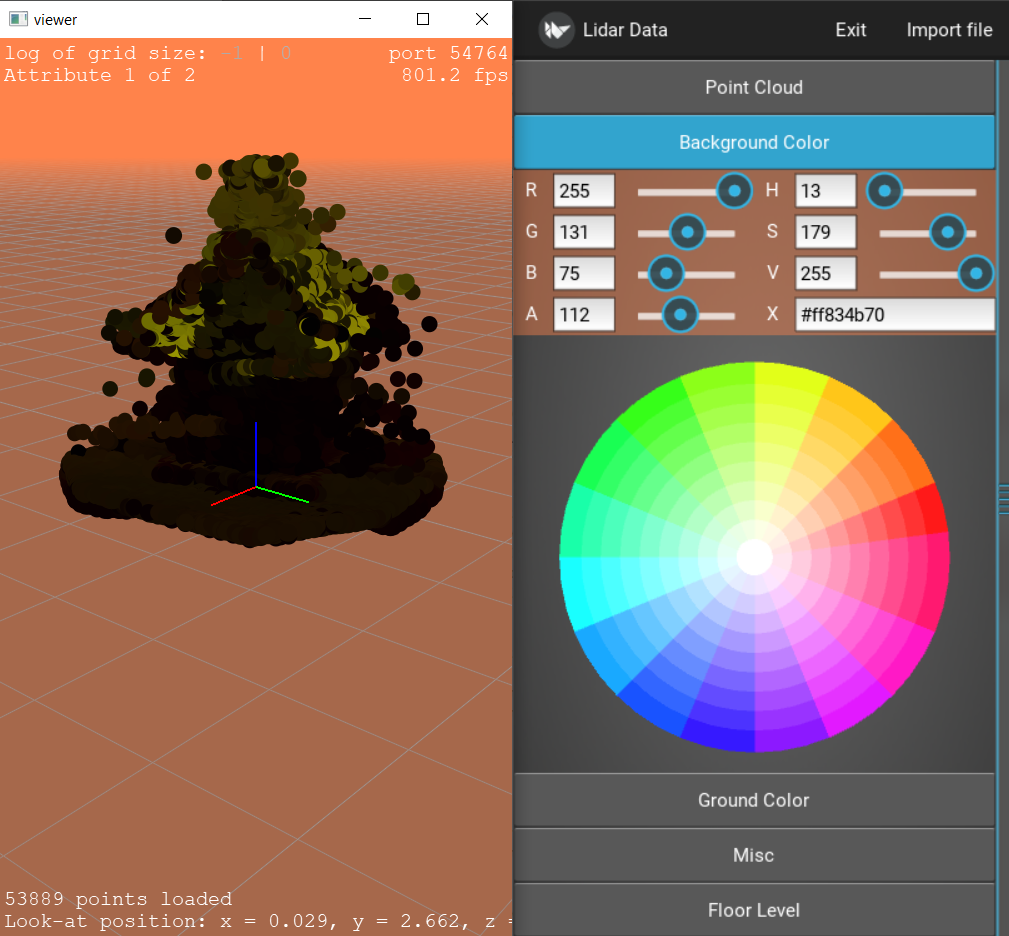
\includegraphics[width=0.45\textwidth]{./media/image11.png}
	\end{subfigure}
~
\end{figure}


%%%%%%%%%%%%%%%%%%%% Figure/Image No: 12 Ends here %%%%%%%%%%%%%%%%%%%%

\begin{Center}
 
\end{Center}\par

\begin{FlushLeft}
\tab \textbf{Figure 11: }Comparisons between expected tool and actual tool.
\end{FlushLeft}\par


\vspace{\baselineskip}

\vspace{\baselineskip}
\textbf{Novelty}\par


\vspace{\baselineskip}
\tab We think that our approach is novel in a significant way because we have not found a tool where it allows you to paint LiDAR points and use this data as an artboard. Also, when we were looking for existing projects that were similar to what we were trying to implement, we could only find one particular project that was remotely close to what we were looking to achieve or even what we have built with the Kivy library. We were able to create a very practical app by combining Python libraries and importing, altering point clouds. The portability is also an asset that has also not been replicated before. This means that the mobile version of this app supports touch features.\par


\vspace{\baselineskip}
\paragraph*{Conclusion}
\addcontentsline{toc}{paragraph}{Conclusion}

\vspace{\baselineskip}
In conclusion, throughout the duration of this project we were able to learn more about 3D reconstruction as well as the usefulness and applications of LiDAR technologies. We presented the theoretical underpinnings of LiDAR and 3D reconstruction by providing a comprehensive description of both of these concepts. In addition, we provided a review of existing methods and algorithms commonly used in the scientific literature. In the methods section we explained the reason behind our choices and ideas about completing the project in terms of data collection, implementation of the app and tools to create the app. Finally, we presented in great detail the implementation of the app with Kivy and Python and the results achieved compared to our stated goal. We are relatively satisfied with the outcome of this project since we were able to bring a novel approach and create a useful tool for LiDAR data analysis while learning about the technology along the way. \par

\paragraph*{References}
\addcontentsline{toc}{paragraph}{References}
\begin{enumerate}
	\item Kada, Martin, and Laurence McKinley. "3D building reconstruction from LiDAR based on a cell decomposition approach." International Archives of Photogrammetry, Remote Sensing and Spatial Information Sciences 38.Part 3 (2009): W4.\par

	\item Forlani, G., Nardinocchi, C., Scaioni, M. et al. Pattern Anal Applic (2006) 8: 357. \href{https://doi.org/10.1007/s10044-005-0018-2}{\textcolor[HTML]{1155CC}{\uline{https://doi.org/10.1007/s10044-005-0018-2}}}\par

	\item Alharthy, Abdullatif. $``$HEURISTIC FILTERING AND 3 D FEATURE EXTRACTION FROM LIDAR DATA.$"$  (2002).\par

	\item Elaksher, Ahmed $\&$  Bethel, James. (2012). Reconstructing 3D buildings from LiDAR data. International Archives of Photogrammetry Remote Sensing and Spatial Information Sciences. 34. \par

	\item Dassot, M., Constant, T. $\&$  Fournier, M. Annals of Forest Science (2011) 68: 959. \href{https://doi.org/10.1007/s13595-011-0102-2}{\textcolor[HTML]{1155CC}{\uline{https://doi.org/10.1007/s13595-011-0102-2}}}\par

	\item  \href{https://medium.com/@d.kudinov}{\textcolor[HTML]{1155CC}{Kudinov}}, D., \href{https://medium.com/@danrhedges}{\textcolor[HTML]{1155CC}{Hedges}}, D., \href{https://medium.com/@omaher}{\textcolor[HTML]{1155CC}{Maher}}}, O. (2018). $``$Reconstructing 3D buildings from aerial LiDAR with AI: details.$"$  [Online]. Available:\par

\href{https://medium.com/geoai/reconstructing-3d-buildings-from-aerial-lidar-with-ai-details-6a81cb3079c0?fbclid=IwAR1ZKNdtPiOevCwwKOWmj19dAKgBaGfOHNnWtI_c9LCyZDXOSGC7m8224W4}{\textcolor[HTML]{1155CC}{\uline{https://medium.com/geoai/reconstructing-3d-buildings-from-aerial-lidar-with-ai-details-6a81cb3079c0?fbclid=IwAR1ZKNdtPiOevCwwKOWmj19dAKgBaGfOHNnWtI\_c9LCyZDXOSGC7m8224W4}}}\par

	\item \textcolor[HTML]{2E414F}{Bizjak, Marko. $``$Reconstruction of Buildings from LiDAR Data.$"$  (2015). \href{http://old.cescg.org/CESCG-2015/papers/Bizjak-3D_reconstruction_of_buildings_from_LiDAR_data.pdf?fbclid=IwAR2lUKTvpC_ArjD28hnbIskxjdsoGpz2de5O_qseWdYGZRGno5QclijNJD4}{\uline{http://old.cescg.org/CESCG-2015/papers/Bizjak-3D\_reconstruction\_of\_buildings\_from\_LiDAR\_data.pdf?fbclid=IwAR2lUKTvpC\_ArjD28hnbIskxjdsoGpz2de5O\_qseWdYGZRGno5QclijNJD4}}}}\par

	\item \textcolor[HTML]{2E414F}{\parbox{\linewidth}{Fayez Tarsha-Kurdi, Tania Landes, Pierre Grussenmeyer. Hough-Transform and Extended RANSAC Algorithms for Automatic Detection of 3D Building Roof Planes from Lidar Data. ISPRS Workshop on Laser Scanning 2007 and SilviLaser 2007, Sep 2007, Espoo, Finland. XXXVI, pp.407-412, 2007. }}}\par

	\item \textcolor[HTML]{333333}{Dassot, M., Constant, T. $\&$  Fournier, M. Annals of Forest Science (2011) 68: 959. \href{https://doi.org/10.1007/s13595-011-0102-2}{\uline{https://doi.org/10.1007/s13595-011-0102-2}}}\par

	\item \textcolor[HTML]{333333}{J. Reitberger, Cl. Schnörr, P. Krzystek, U. Stilla, 3D segmentation of single trees exploiting full waveform LIDAR data, ISPRS Journal of Photogrammetry and Remote Sensing, Volume 64, Issue 6, 2009, Pages 561-574, ISSN 0924-2716, \href{https://doi.org/10.1016/j.isprsjprs.2009.04.002}{\uline{https://doi.org/10.1016/j.isprsjprs.2009.04.002}}.}\par

	\item \textcolor[HTML]{333333}{Li, M., Cheng, L., Gong, J. et al. Sci. China Ser. E-Technol. Sci. (2008) 51(Suppl 2): 133. \href{https://doi.org/10.1007/s11431-008-6014-1}{\uline{https://doi.org/10.1007/s11431-008-6014-1}}}\par

	\item \textcolor[HTML]{222222}{\parbox{\linewidth}{Carter, Jamie; Keil Schmid; Kirk Waters; Lindy Betzhold; Brian Hadley; Rebecca Mataosky; Jennifer Halleran (2012). \href{https://coast.noaa.gov/data/digitalcoast/pdf/lidar-101.pdf}{}}\parbox{\linewidth}{\uline{"Lidar 101: An Introduction to Lidar Technology, Data, and Applications." (NOAA) Coastal Services Center"}}}} (PDF). \textit{Coast.noaaa.gov}. p. 14. Retrieved 2017-02-11.}}\par

	\item \textcolor[HTML]{333333}{DEM, DSM $\&$  DTM Differences - A Look at Elevation Models in GIS.}\par

\href{https://gisgeography.com/dem-dsm-dtm-differences/}{\textcolor[HTML]{1155CC}{\uline{https://gisgeography.com/dem-dsm-dtm-differences/}}}\par


\vspace{\baselineskip}
	\item \textcolor[HTML]{2E414F}{\parbox{\linewidth}{Morgenroth, Justin $\&$  Gomez, Christopher. (2013). Assessment of tree structure using a 3D image analysis technique—A proof of concept. Urban Forestry $\&$  Urban Greening. 13. 10.1016/j.ufug.2013.10.005. }}}\par

	\item \textcolor[HTML]{2E414F}{\parbox{\linewidth}{Liang Cheng, Lihua Tong, Yanming Chen, Wen Zhang, Jie Shan, Yongxue Liu, Manchun Li. Integration of LiDAR data and optical multi-view images for 3D reconstruction of building roofs, Optics and Lasers in Engineering, Volume 51, Issue 4, 2013, Pages 493-502, ISSN 0143-8166,}}}
\end{enumerate}\par

\begin{adjustwidth}{0.5in}{0.0in}
\href{https://doi.org/10.1016/j.optlaseng.2012.10.010}{\textcolor[HTML]{1155CC}{\uline{https://doi.org/10.1016/j.optlaseng.2012.10.010}}.}}\par

\end{adjustwidth}


\vspace{\baselineskip}
\begin{adjustwidth}{0.5in}{0.0in}
\textcolor[HTML]{2E414F}{Kivy, \href{https://kivy.org/#home}{\uline{https://kivy.org/$\#$ home}}}}\par

\end{adjustwidth}

\begin{adjustwidth}{0.5in}{0.0in}
\textcolor[HTML]{2E414F}{Python, \href{https://www.python.org/}{\uline{https://www.python.org/}}}}\par

\end{adjustwidth}

\begin{adjustwidth}{0.5in}{0.0in}
\textcolor[HTML]{2E414F}{PPTK, \href{https://heremaps.github.io/pptk/}{\uline{https://heremaps.github.io/pptk/}}}}\par

\end{adjustwidth}


\printbibliography
\end{document}